
\section{Algorithm comparison}

\Warning[TODO]{ Compare with a simple top-list? Or something else easy? }

\begin{enumerate}
    \item Time to optimize for different datasets
    \item Time to recommend given optimized parameters
    \item Performance of recommendations given optimized parameters
\end{enumerate}

\begin{table}[h!]
    \centering
    \begin{tabular}{| c | c | c | c | c |}
        \hline
        \textbf{}               & \multicolumn{2}{c|}{\textbf{katz-eig}} & \multicolumn{2}{c|}{\textbf{link-analysis}} \\ \hline
        \textit{alphaS}         & 41.876401     & 9.106161         & 26.978338     & 0.877453      \\ \hline
        \textit{eswc2015books}  & 1.871681      & 0.023562         & 3.245297      & 0.026975      \\ \hline
        \textit{eswc2015movies} & 52.749416     & 5.194185         & x             & x             \\ \hline
        \textit{eswc2015music}  & 141.664568    & 5.769257         & x             & x             \\ \hline
        \textit{movielens1m}    & 31.249456     & 0.190485         & 244.484291    & 58.205089     \\ \hline
        \textit{romeo}          & 3.781222      & 0.012321         & 81.478788     & 4.675901      \\ \hline
    \end{tabular}
    \caption{Runtime for optimizing the different algorithms for the different datasets. Uses the fastest optimization strategy.}
    \label{tab:alg_full_time}
\end{table}

\begin{table}[h!]
    \centering
    \begin{tabular}{| c | c | c | c | c |}
        \hline
        \textbf{}               & \multicolumn{2}{c|}{\textbf{katz-eig}} & \multicolumn{2}{c|}{\textbf{link-analysis}} \\ \hline
        \textit{alphaS}         & 3.434409 s & 1.038829 & 10.307018 s  & 0.068634       \\ \hline
        \textit{eswc2015books}  & 0.027989 s & 0.004293 & 0.720686 s   & 0.016339       \\ \hline
        \textit{eswc2015movies} & 1.382029 s & 0.516727 & x            & x              \\ \hline
        \textit{eswc2015music}  & 2.001985 s & 0.159226 & x            & x              \\ \hline
        \textit{movielens1m}    & 1.410586 s & 0.107071 & 154.404908 s & 18.179708      \\ \hline
        \textit{romeo}          & 0.216897 s & 0.032052 & 40.477119 s  & 0.114363       \\ \hline
    \end{tabular}
    \caption{Runtime of the algorithms using the full interaction history using the optimized parameters given in \appendixref{app:opt_params}.}
    \label{tab:alg_full_time}
\end{table}


\begin{table}[h!]
    \centering
    \begin{tabular}{| c | c | c | }
        \hline
        \textbf{}               & \textbf{katz-eig} & \textbf{link-analysis} \\ \hline
        \textit{alphaS}         & 0.002174          & \textbf{0.003208}      \\ \hline
        \textit{eswc2015books}  & 0.020102          & \textbf{0.023537}      \\ \hline
        \textit{eswc2015movies} & \textbf{0.048456} & x                      \\ \hline
        \textit{eswc2015music}  & \textbf{0.054448} & x                      \\ \hline
        \textit{movielens1m}    & \textbf{0.124839} & 0.090044               \\ \hline
        \textit{romeo}          & \textbf{0.145914} & 0.134655               \\ \hline
    \end{tabular}
    \caption{Performance on \textit{F-measure} of the different algorithms using the optimized parameters given in \appendixref{app:opt_params}.}
    \label{tab:alg_full_perf}
\end{table}

%\begin{figure}[h!]
    %\centering
    %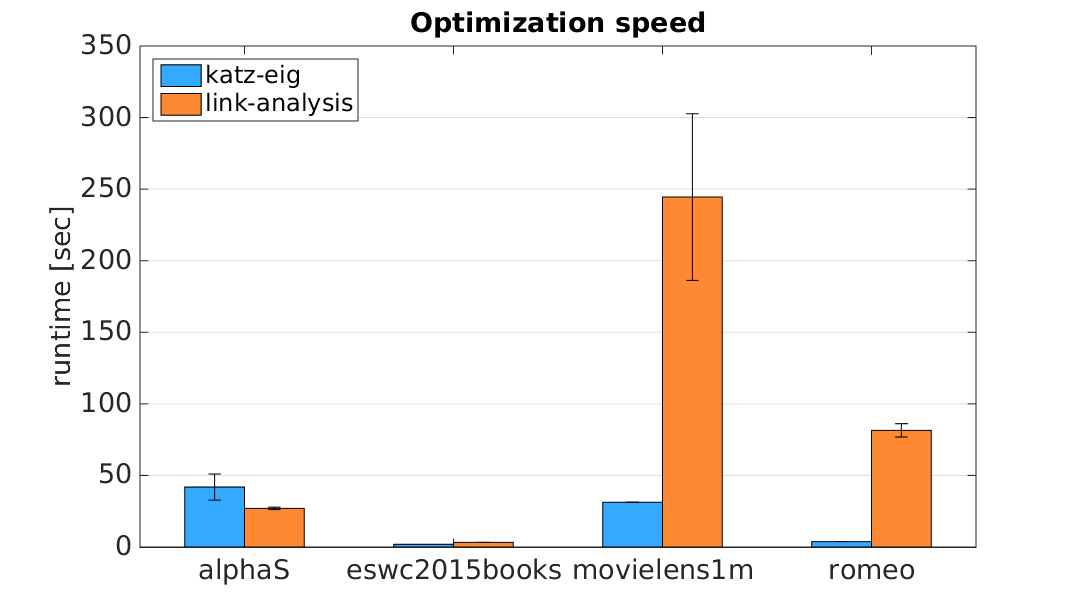
\includegraphics[width=0.9\textwidth]{fig/comp/comp_rec_opt_time.png}
    %\caption{totod}
%\end{figure}

\begin{figure}[h!]
    \begin{subfigure}[h!]{0.5\textwidth}
        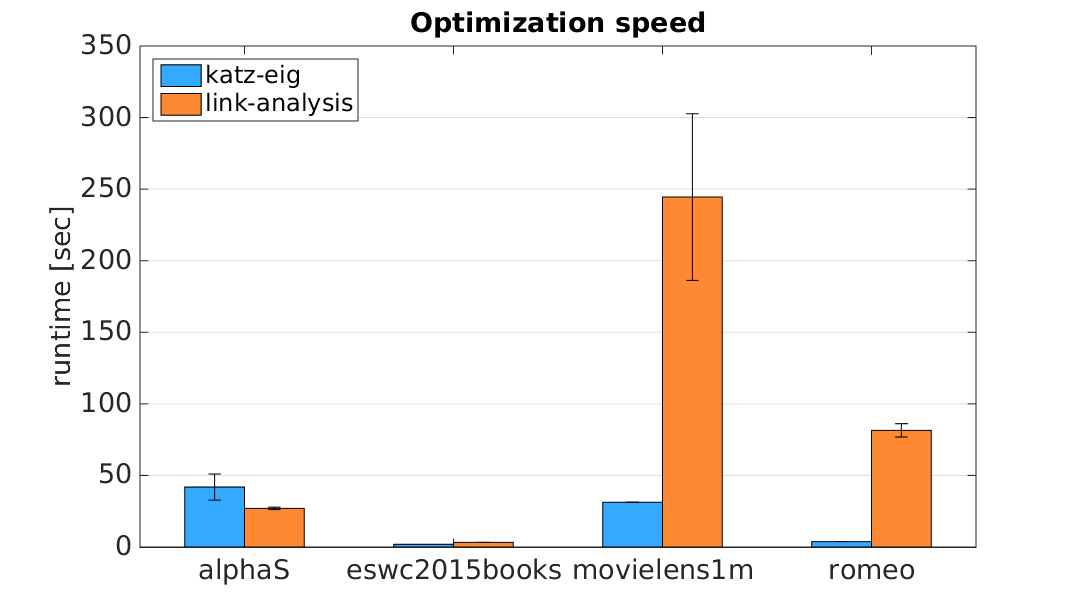
\includegraphics[width=\textwidth]{fig/comp/comp_rec_opt_time.png}
        \caption{}
        %\label{fig:rec_speed}
    \end{subfigure}
    ~
    \begin{subfigure}[h!]{0.5\textwidth}
        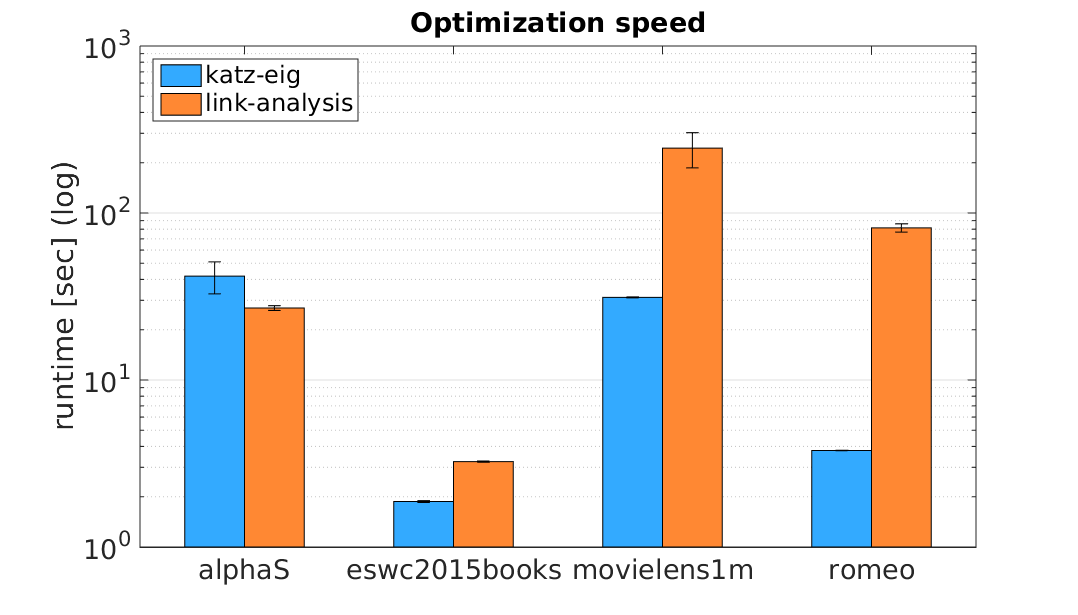
\includegraphics[width=\textwidth]{fig/comp/comp_rec_opt_time_log.png}
        \caption{}
        %\label{fig:rec_speed_log}
    \end{subfigure}
    \caption{TODO}
\end{figure}

\begin{figure}[h!]
    \centering
    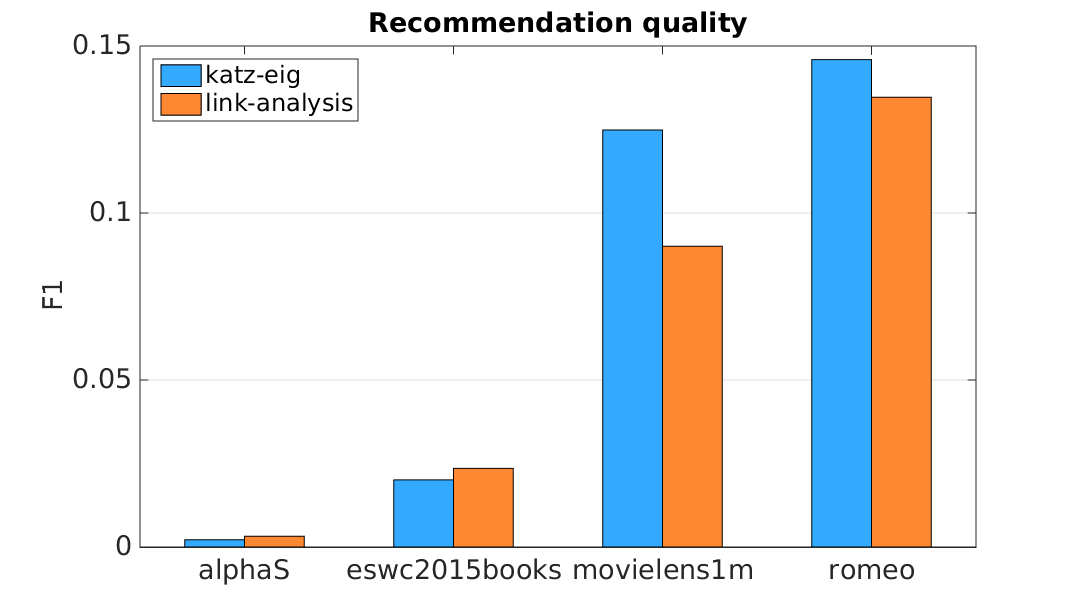
\includegraphics[width=0.9\textwidth]{fig/comp/comp_rec_quality.png}
    \caption{Comparison of the recommendation quality given from the different algorithms, given the optimized parameters specified in \appendixref{app:opt_params}.}
\end{figure}

\begin{figure}[h!]
    \begin{subfigure}[h!]{0.5\textwidth}
        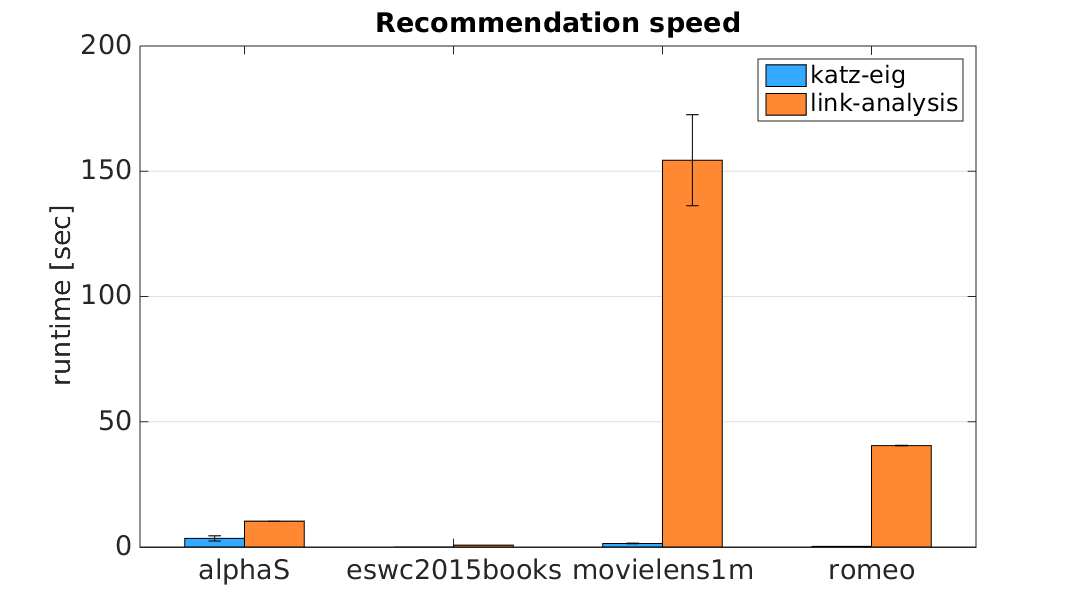
\includegraphics[width=\textwidth]{fig/comp/comp_rec_speed.png}
        \caption{}
        %\label{fig:rec_speed}
    \end{subfigure}
    ~
    \begin{subfigure}[h!]{0.5\textwidth}
        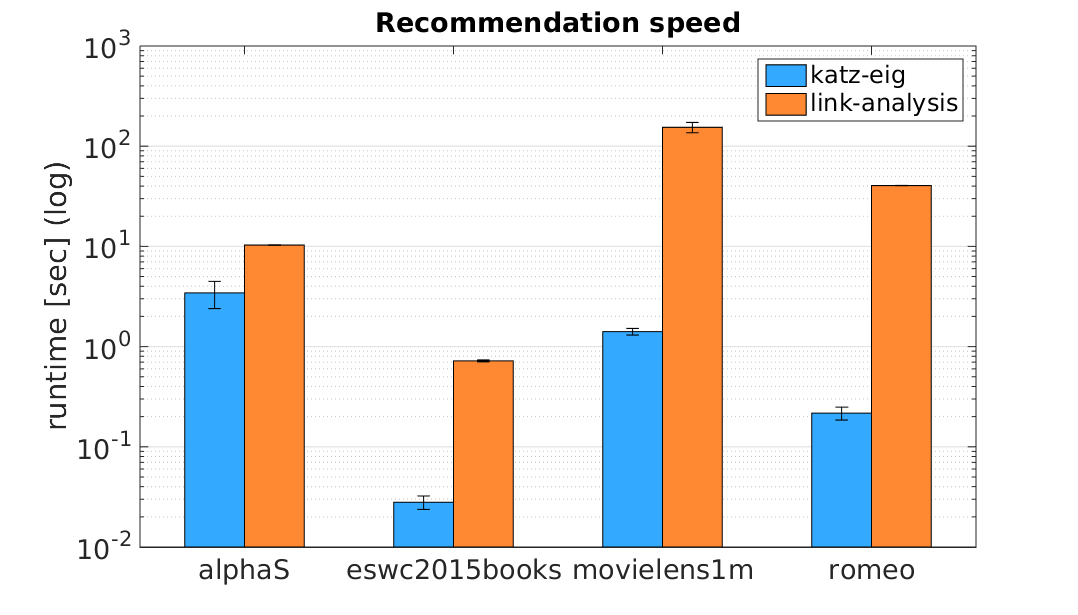
\includegraphics[width=\textwidth]{fig/comp/comp_rec_speed_log.png}
        \caption{}
        %\label{fig:rec_speed_log}
    \end{subfigure}
    \caption{Comparison of the runtime of generating recommendations for the full dataset for the different algorithms. (b) shows the speed with logarithmic y-axis. Both plots include the standard deviation of the 10 runs made.}
\end{figure}

